%%Plantilla para la entrega de trabajos
\documentclass{article}
\usepackage{graphicx} %%Estos son paquetes de imagenes
\usepackage[utf8]{inputenc} %%Paquete para simbolos utf8
\usepackage[T1]{fontenc} %%Paquete para la impresion de simbolos y carácteres
\usepackage{hyperref} %%Paquete para manejar hipervinculos
\usepackage[spanish]{babel} %%paquete para el lenguaje
\usepackage{enumerate}
\usepackage{anysize} %%Margenes
\usepackage{amsmath}
\usepackage{amssymb}
\usepackage[usenames]{color}
\usepackage{float}
\author{Barajas Figueroa José de Jesús}
%%\setlength{\parindent}{1cm} %%Especificar sangrias

\begin{document}
\marginsize{3cm}{2cm}{2cm}{2cm} 
\begin{titlepage} %%Inicio de página de presentación
\begin{center}
    
\begin{figure}[ht]
\begin{center}

\includegraphics[width=1.8in]{./img/unamlogo.png}
\end{center}
\end{figure}

\begin{center}
  {\Large \textbf{
      \vspace*{.5in}   
UNIVERSIDAD NACIONAL AUTONOMA DE MEXICO\\
\vspace*{.3in}
FACULTAD DE CIENCIAS}}\\
\vspace*{.3in}
Proyecto Final\\%%nombre del trabajo
\vspace*{.3in}
Fundamentos de Bases de Datos\\
\vspace*{.3in}
Profesor: Gerardo Aviles Rosas\\
Ayudante: Maria del Pilar Hernández Bastida\\
Ayudante: Eduardo \\
Ayudamte: Eduardo \\
\vspace*{.3in}

Barajas Figueroa José de Jesús\\
Diana Ramirez Garcia\\
\vspace*{.3in}
2019-1 \\%%Fecha
\begin{figure}[H]
\begin{center}

\includegraphics[width=2.5in]{./img/logo.png}
\end{center}
\end{figure}

    
\end{center}
\end{center}
\end{titlepage}
\section{Diagrama E/R}

El primer boceto de el diagrama lo hicimos prácticamente considerando las entidades y relaciones que nos proporcionaban de manera casi literal, esto para ir tomando consideraciones que de primer mano no son tan aproximadas como el diagrama final que queremos, por ahora creo que nos tenemos que concentrar en guardar lo mas posible la integridad referencial.\\ 
\begin{figure}[H]
\begin{center}
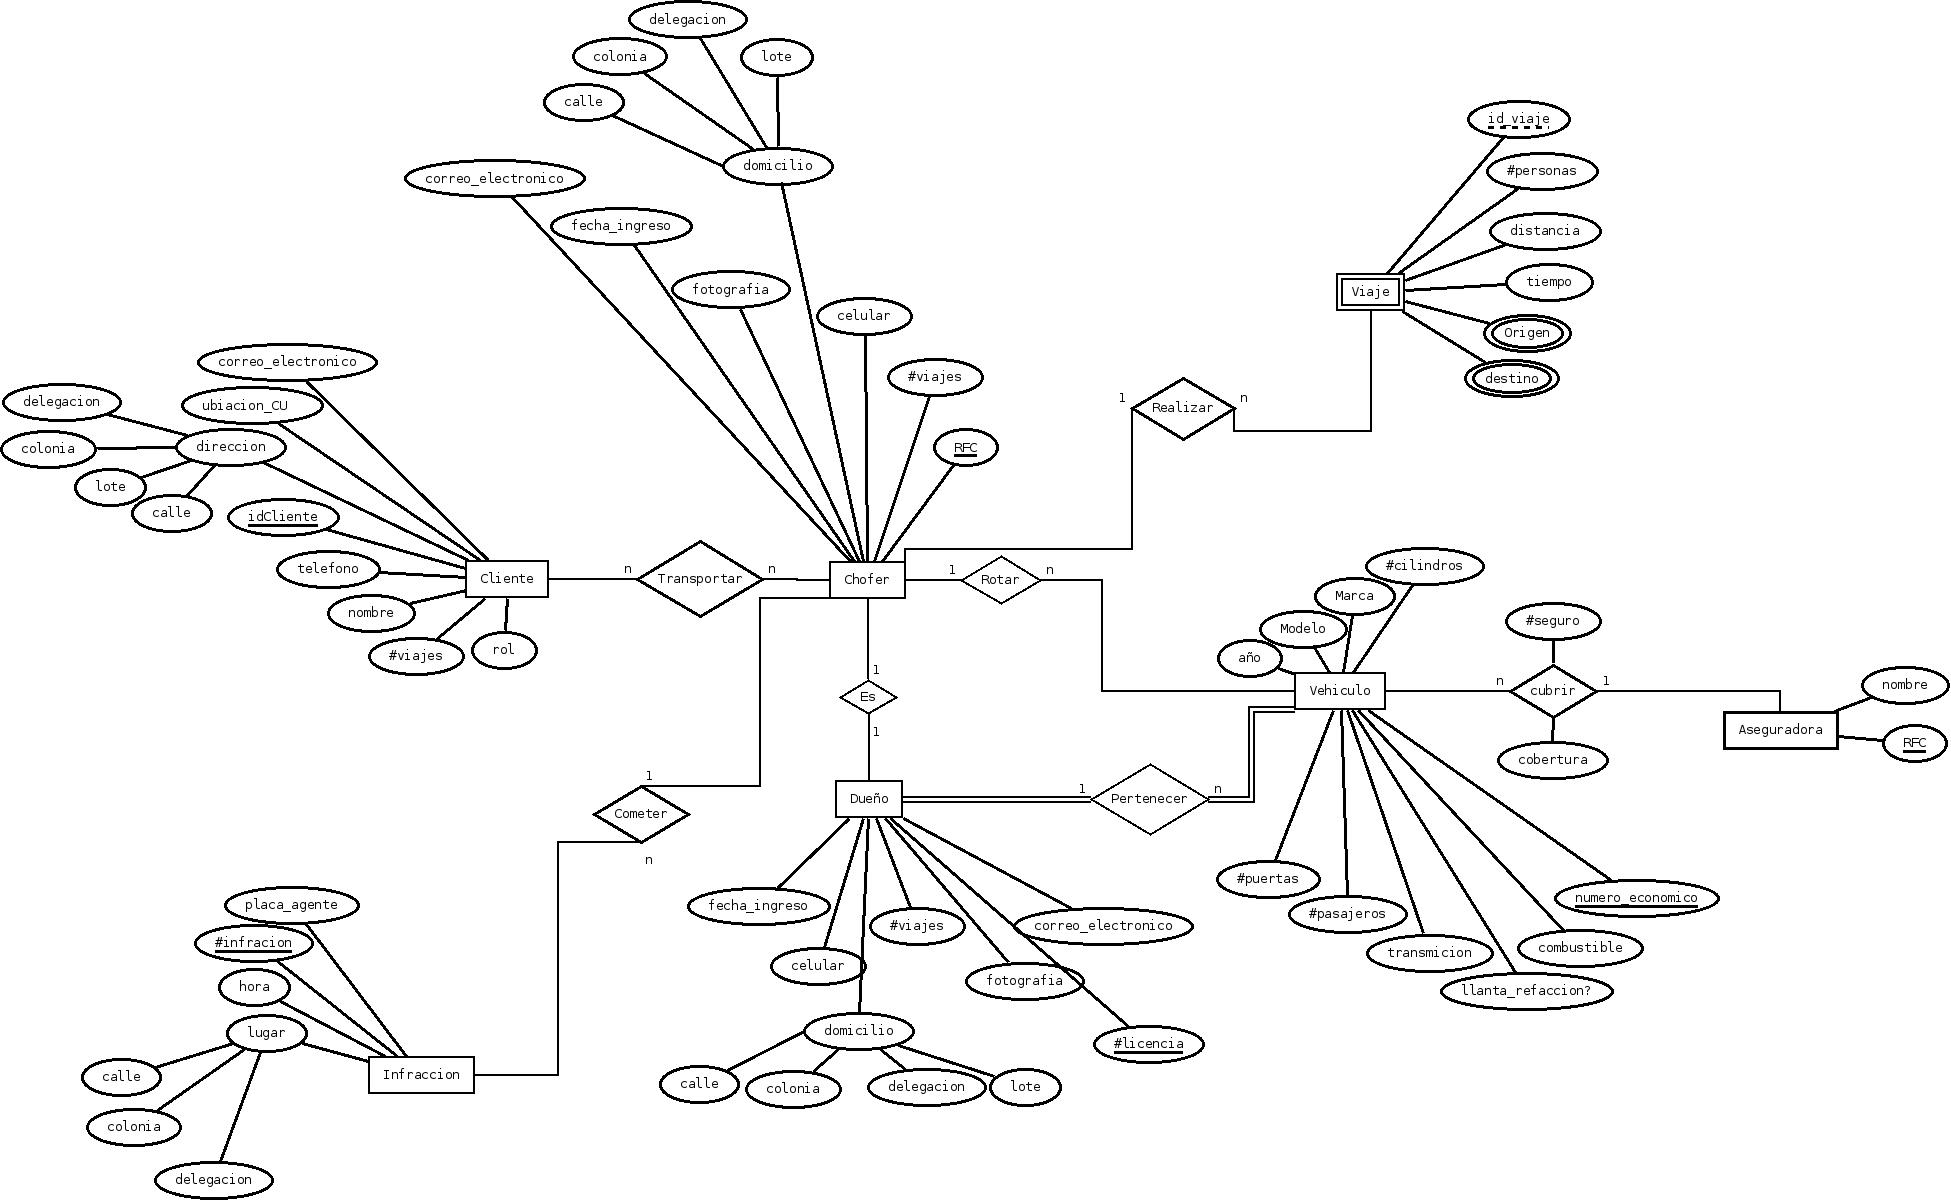
\includegraphics[width=5in]{./img/R_boceto1.jpeg}
\caption{Primer revisión 12-noviembre-2018}
\end{center}
\end{figure}

Aqui podemos observar las primeras modificaciones echas al diagrama, en primera instancia, convertimos la relacion transportar en una relacion ternaria, con cliente, viaje y chofer, ya que anteriormente teniamos viaje y clientes separados, no teniamos una forma de crear un vínculo entre el viaje y el cliente, a su vez, dejamos intactas las relaciones, perteneces, cubrir, manejar y cometer. Sin embargo aun tenemos un poco de duas a cerca de como se quiera manejar el descuento de cada viaje.\\

\begin{figure}[H]
\begin{center}
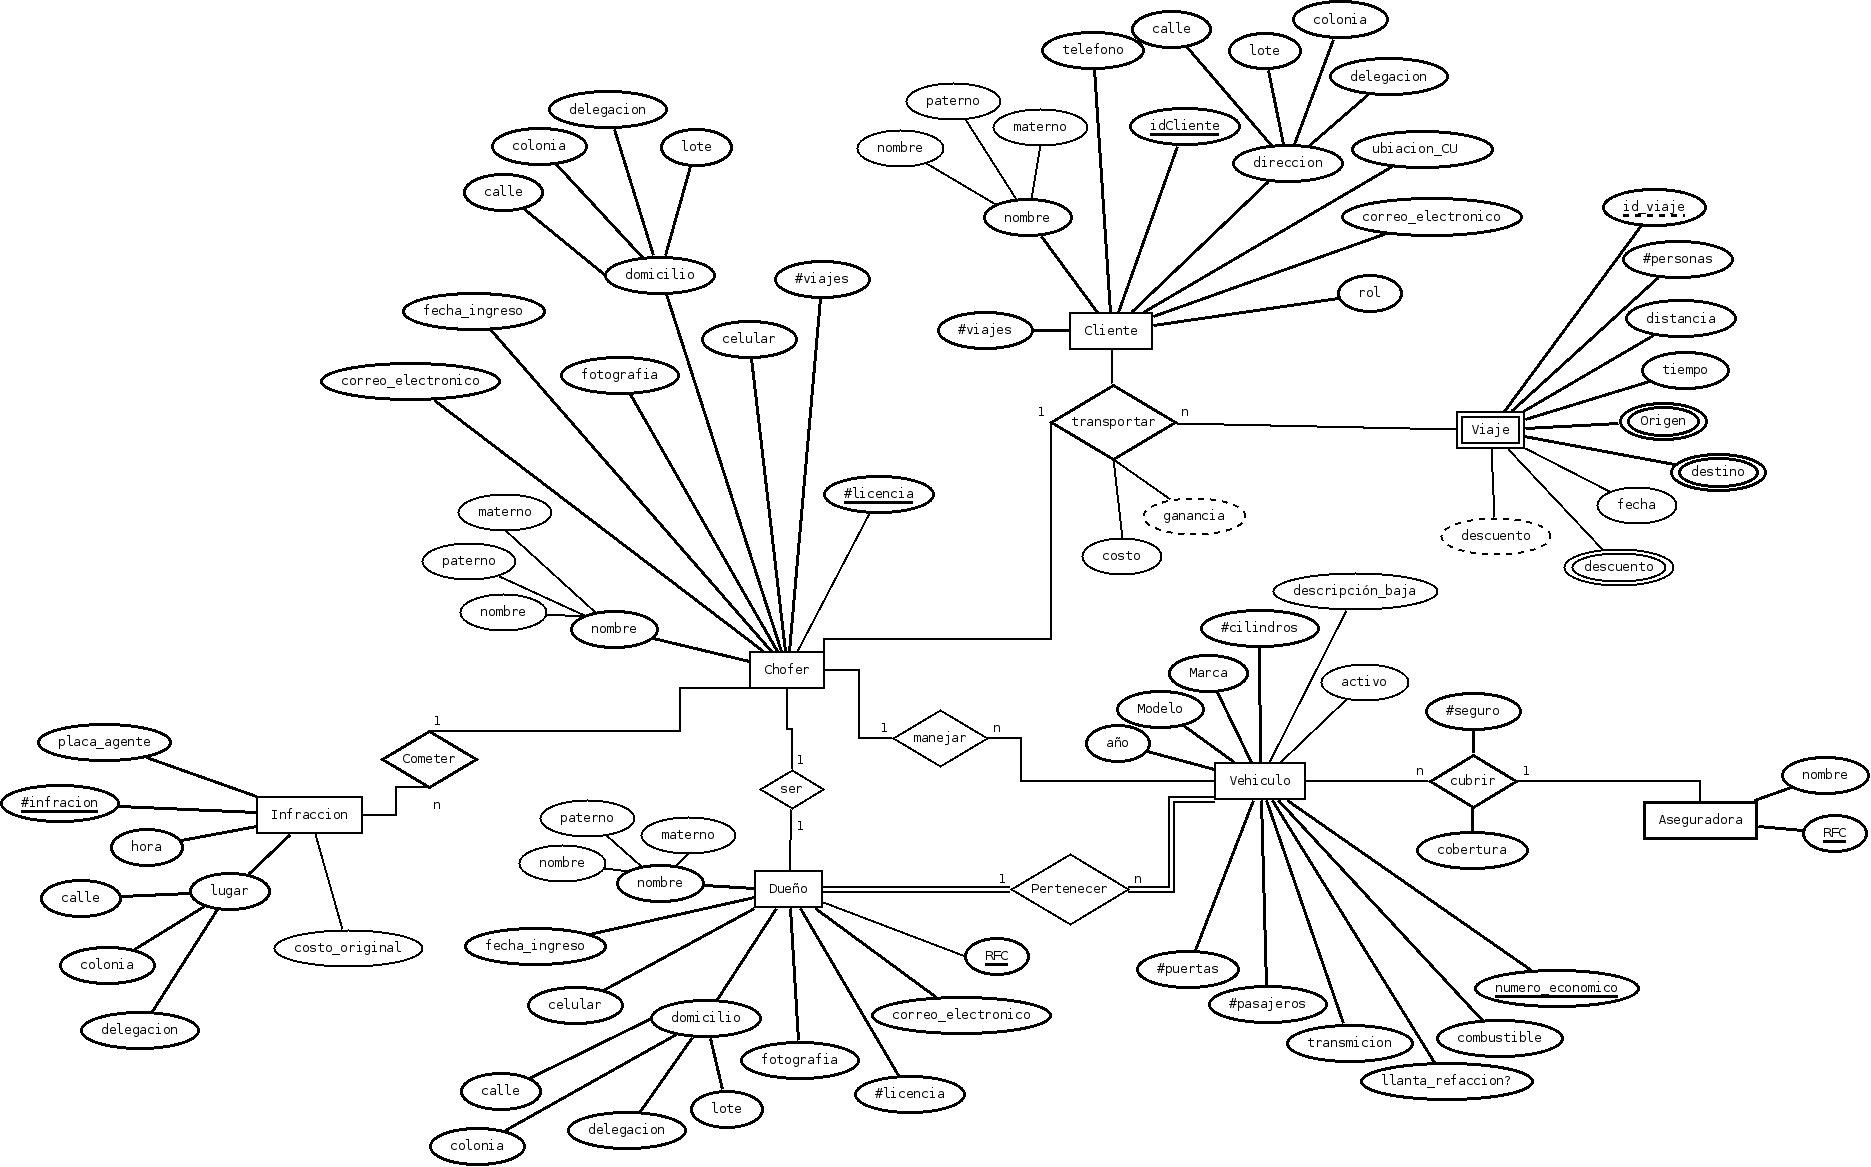
\includegraphics[width=5in]{./img/R_boceto2.jpeg}
\caption{Segunda revisión 19-Noviembre-2018}
\end{center}
\end{figure}


\begin{figure}[H]
\begin{center}
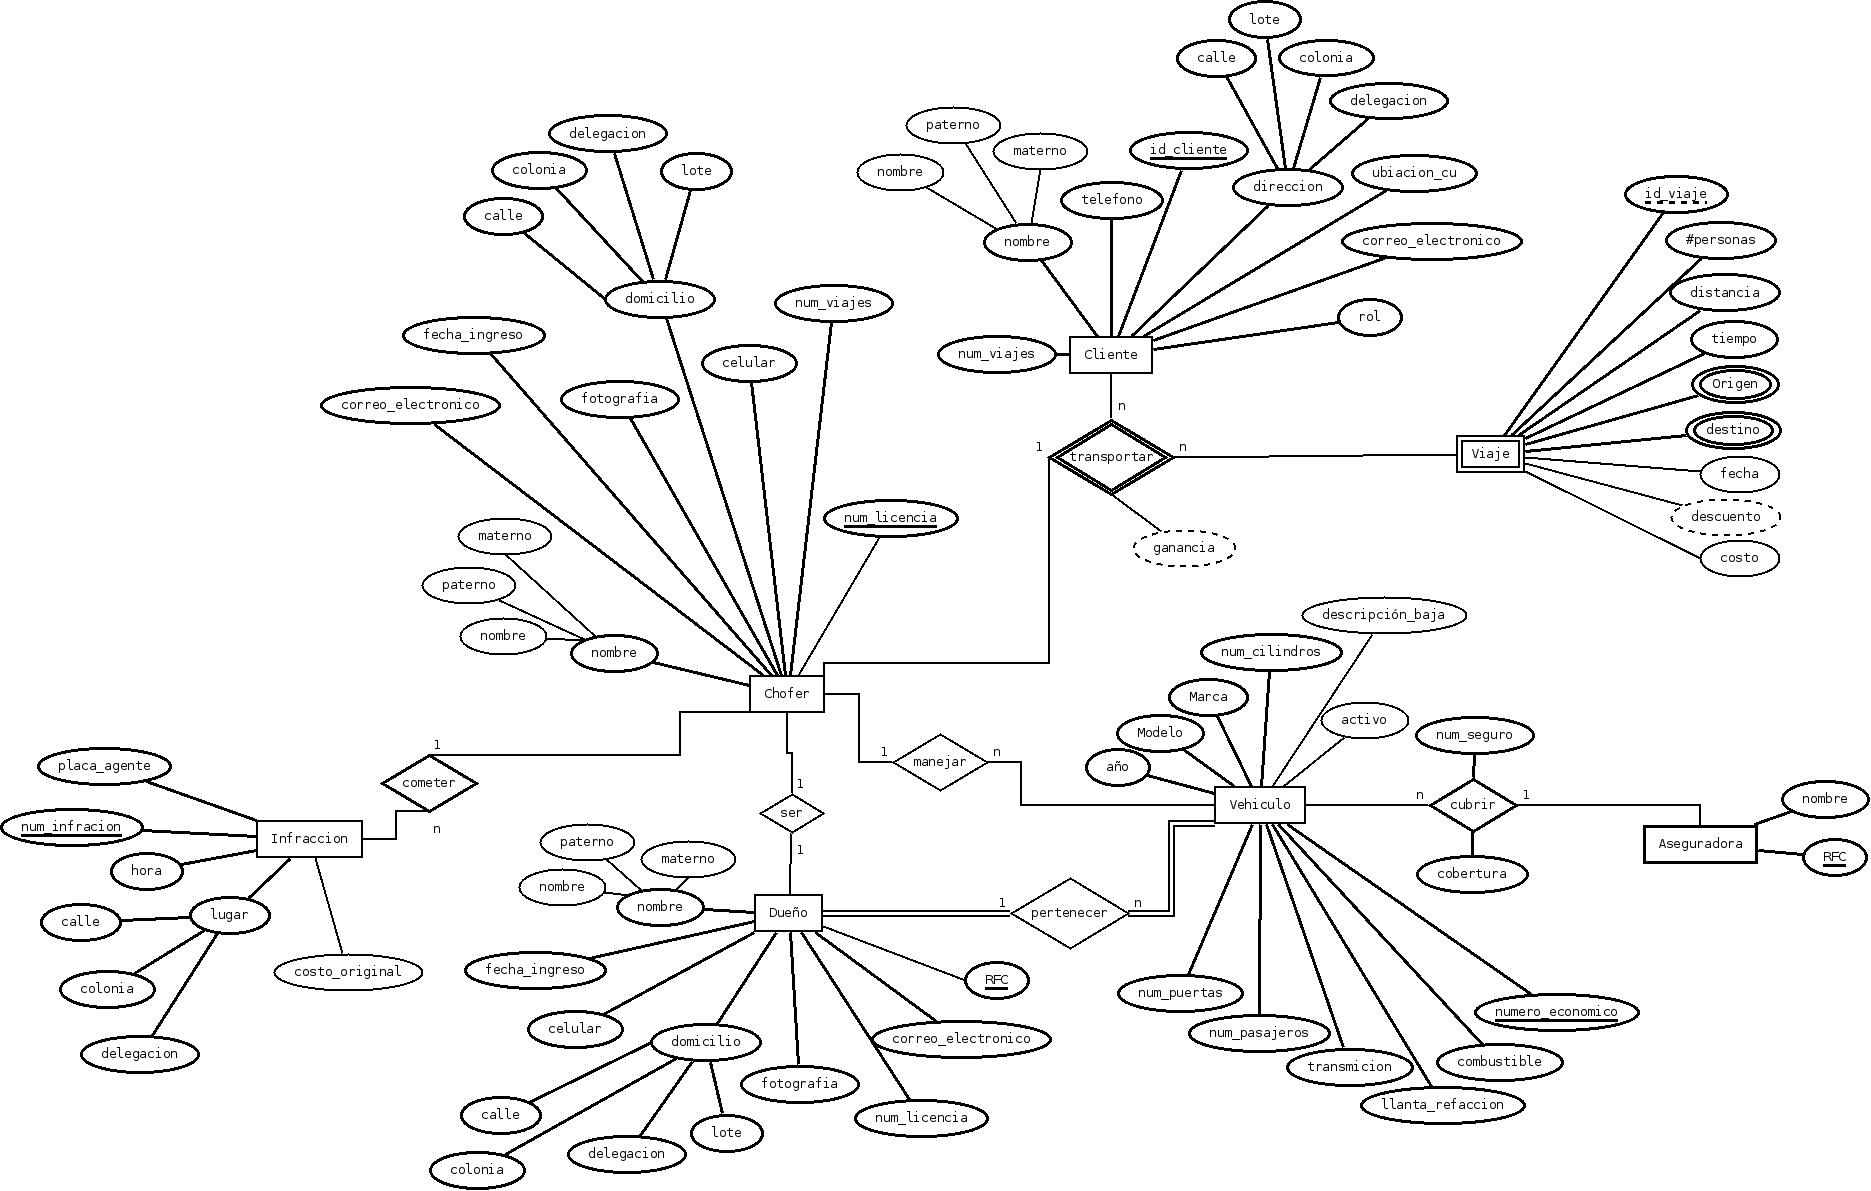
\includegraphics[width=5in]{./img/R_boceto3.jpeg}
\caption{Diagrama E/R final. 21-Noviembre-2018 }
\end{center}
\end{figure}

en este diagrama final, cambiamos todos los nombres de atributos que tenian simbolos especiales como \# o ?, definimos tambien la relacion débil,  quitamos un atributos, por último decidimos tomar a descuento como un atributo calculado.\\

\Section{Diagrama Relacional}

Una vez completado el diagram entidad relación, se comenzo con la transformacion sintáctica a un diagrama Relacional, se aprecia el como se desaparecen los atributos calculados(datos que podemos obtener en tiempo constante sin necesidad de ocupar espacio en la base de datos). Como es el caso de descuento, ganancia y costo, y nuestro atributos multivaluados generan nuevas tablas como lo son origen y destino\\

\begin{figure}[H]
\begin{center}
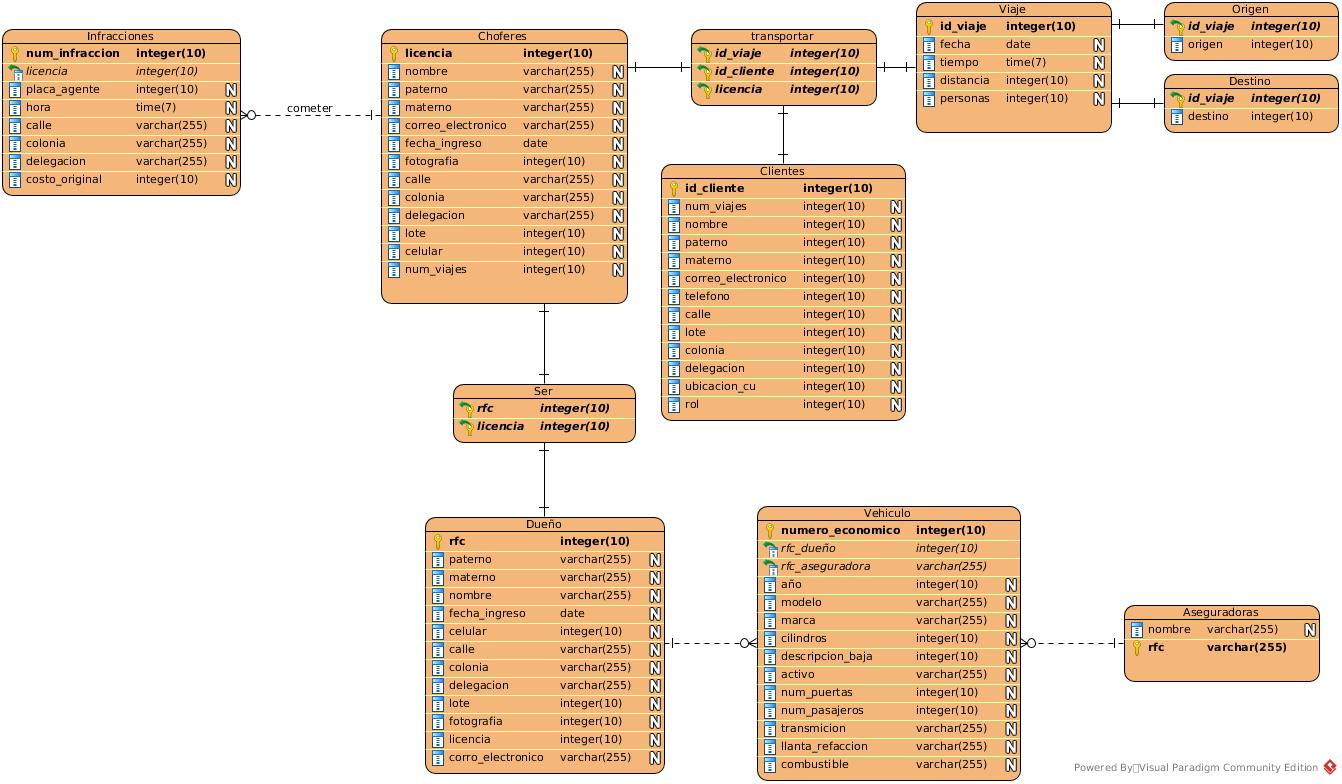
\includegraphics[width=5in]{./img/relacional.jpg}
\caption{Diagrama relacional 21-Noviembre-2018}
\end{center}
\end{figure}



\section{Referencias}

\end{document}
